\setchapterimage{Fond_SLCI.png}
\setchapterpreamble[u]{\margintoc}
\setcounter{chapter}{1}

\chapter{Correction des SLCI}

\marginnote[3cm]{
\UPSTIcompetence[2]{C1-02}
\UPSTIcompetence[2]{C2-04}
}

%\marginnote[4cm]{\textbf{Qui}, \textit{Quoi}, Où.}
\marginnote[4cm]{\textbf{Frédéric Mazet}, \textit{Cours d'automatique de deuxième année}, Lycée Dumont Durville, Toulon.}
\marginnote[4cm]{\textbf{Florestan Mathurin}, \textit{Correction des SLCI}, Lycée Bellevue, Toulouse, \url{http://florestan.mathurin.free.fr/}.}


\section{Pourquoi corriger un système ?}



Souvent évoqué en lors de l'étude des systèmes asservis, regardons ce qui se cache derrière le bloc correcteur. On peut le considérer comme la partie intelligente du système car de sa part position dans l'architecture d'un système il reçoit l'image de l'écart entre la cosigne et la sortie du système. En fonction de cet écart, en fonction de ses << capacités >> va permettre d'améliorer les performances du système. 

Sur la figure ci-contre est tracée en gris la réponse indicielle d'un système non corrigé et en noir la réponse indicielle du système corrigé. On observe que le système corrigé est :
\begin{itemize}
\item plus précis;
\item plus amorti;
\item plus rapide. 
\end{itemize}
L'objectif du correcteur est donc d'améliorer les caractéristiques tout en assurant la stabilité su système.




\begin{resultat} 
\begin{itemize}
\item D'après les résultats sur la stabilité des systèmes asservis :
\begin{itemize}
\item le correcteur doit permettre d'avoir des marges de gains suffisantes.
\end{itemize}
\item D'après les résultats sur la rapidité des systèmes asservis :
\begin{itemize}
\item le correcteur doit permettre d'augmenter le gain dans le but d'avoir une pulsation de coupure à \SI{0}{dB} la plus grande possible (pour la FTBO).
\end{itemize}
\item D'après les résultats sur la précision des systèmes asservis :
\begin{itemize}
\item le correcteur doit permettre d'augmenter le gain statique de la boucle ouverte pour assurer une bonne précision du système (et d’éventuellement augmenter la classe).
\end{itemize}
\end{itemize}
Au vue de ces conclusions, le choix d'un correcteur se fera dans le domaine fréquentiel en utilisant le diagramme de Bode. 
\end{resultat}


\section{Le correcteur proportionnel}

\begin{defi}[Correcteur P]
Le correcteur proportionnel a pour fonction de transfert $C(p)=K$.
\end{defi}

Prenons le cas d'un système du second ordre bouclé ($K=15$, $\xi=3$, $\omega=1$).

\noindent
\begin{minipage}[c]{.46\linewidth}
\begin{center}
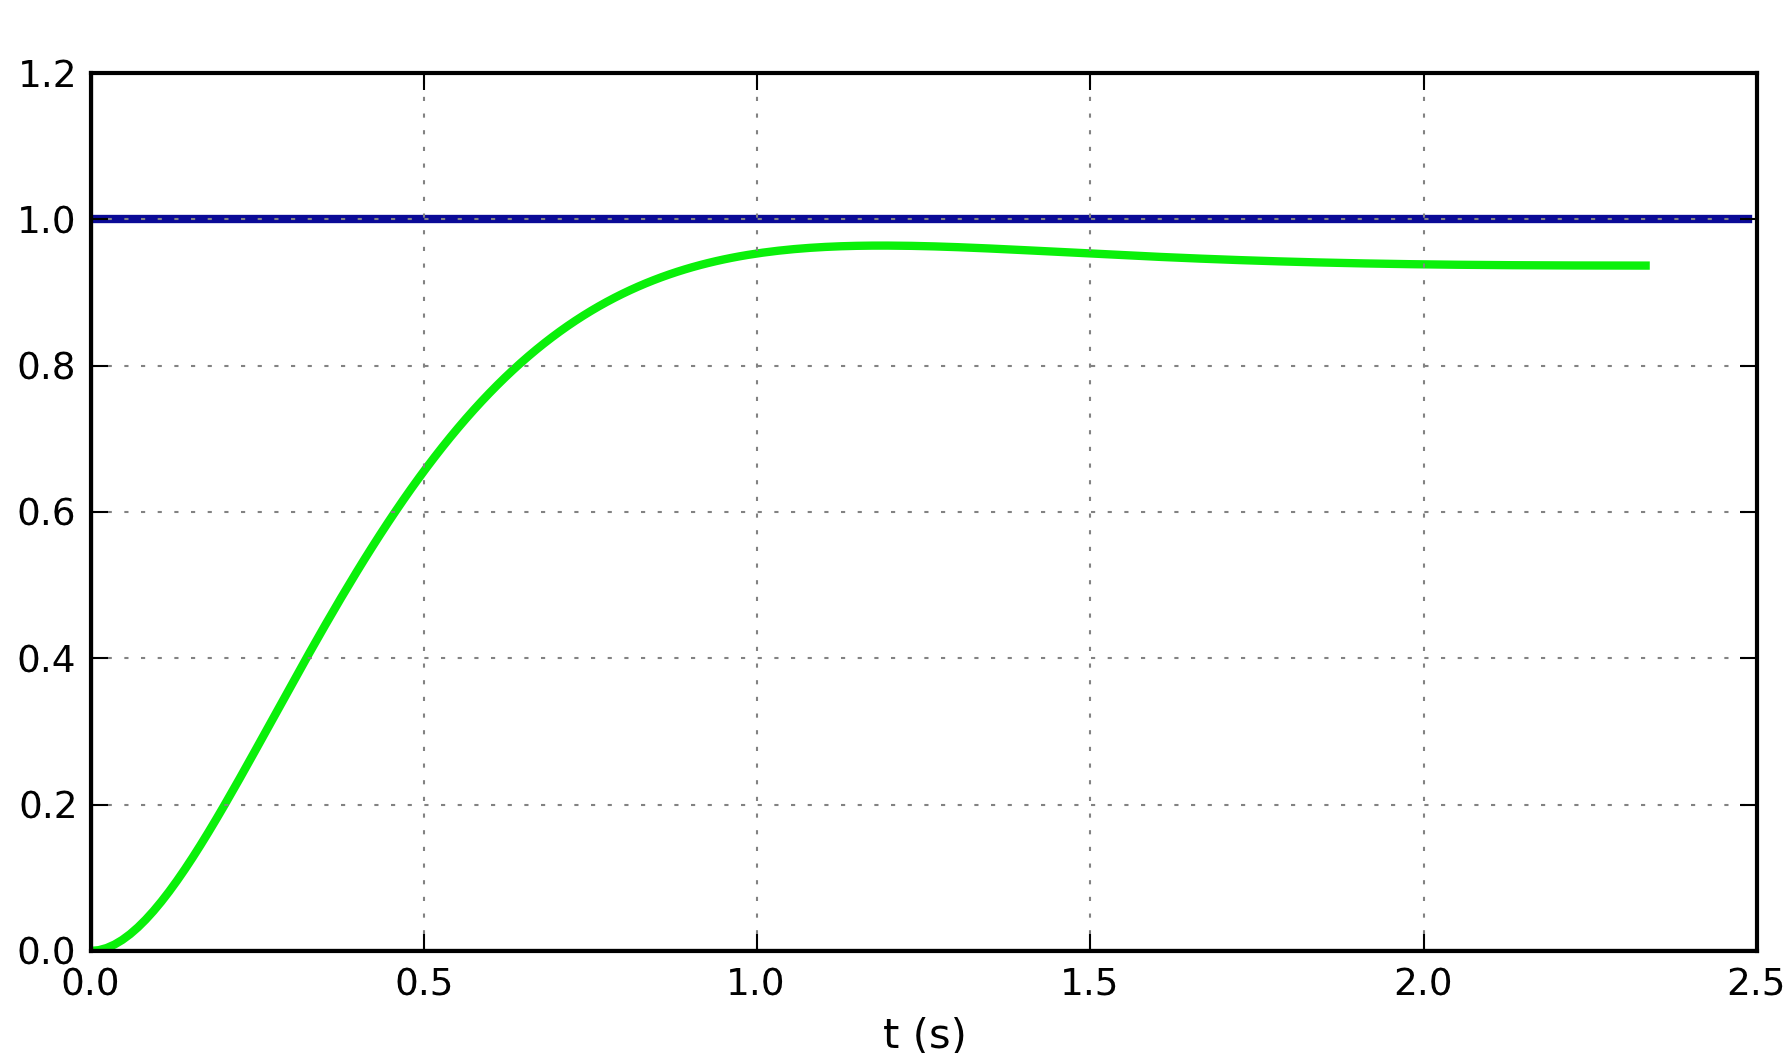
\includegraphics[width=\linewidth]{fig_04a}

$\text{T}_{5\%}$ : \SI{0,781}{s} -- Écart statique : 0,07
\end{center}

\end{minipage} \hfill
\begin{minipage}[c]{.46\linewidth}
\begin{center}
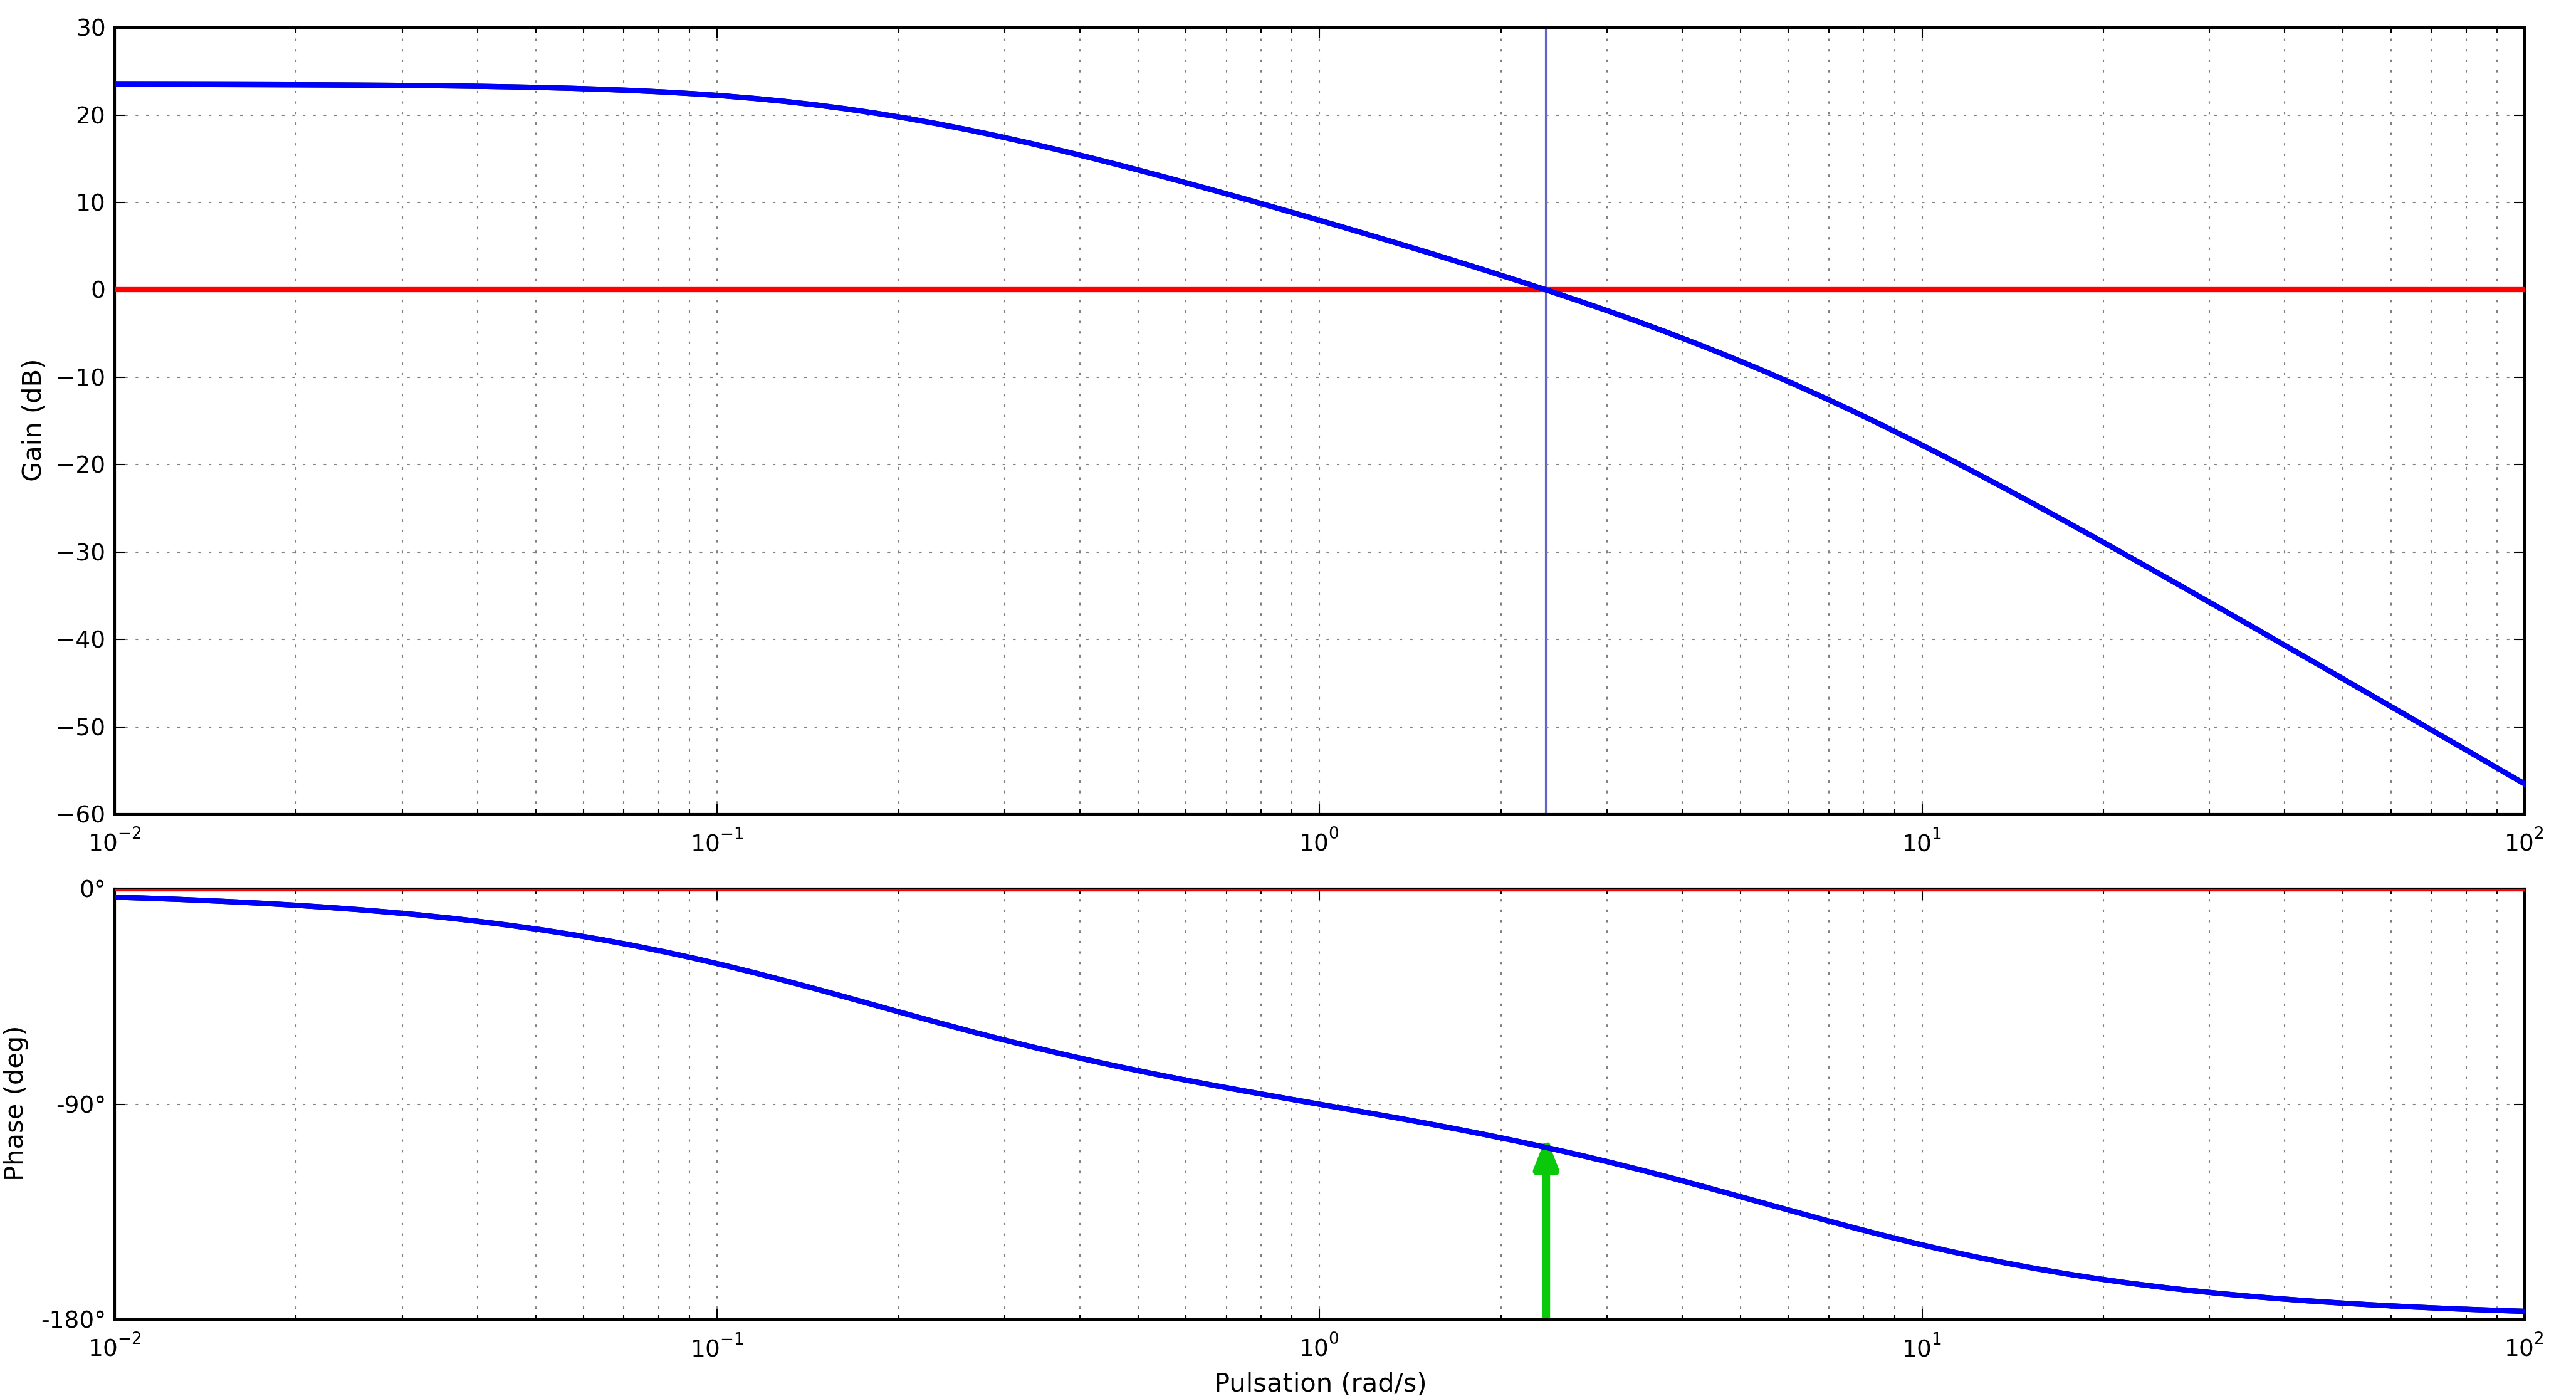
\includegraphics[width=\linewidth]{fig_04b}

Marge de phase 71,94 \degres
\end{center}
\end{minipage} 


\noindent
\begin{minipage}[c]{.46\linewidth}
\begin{center}
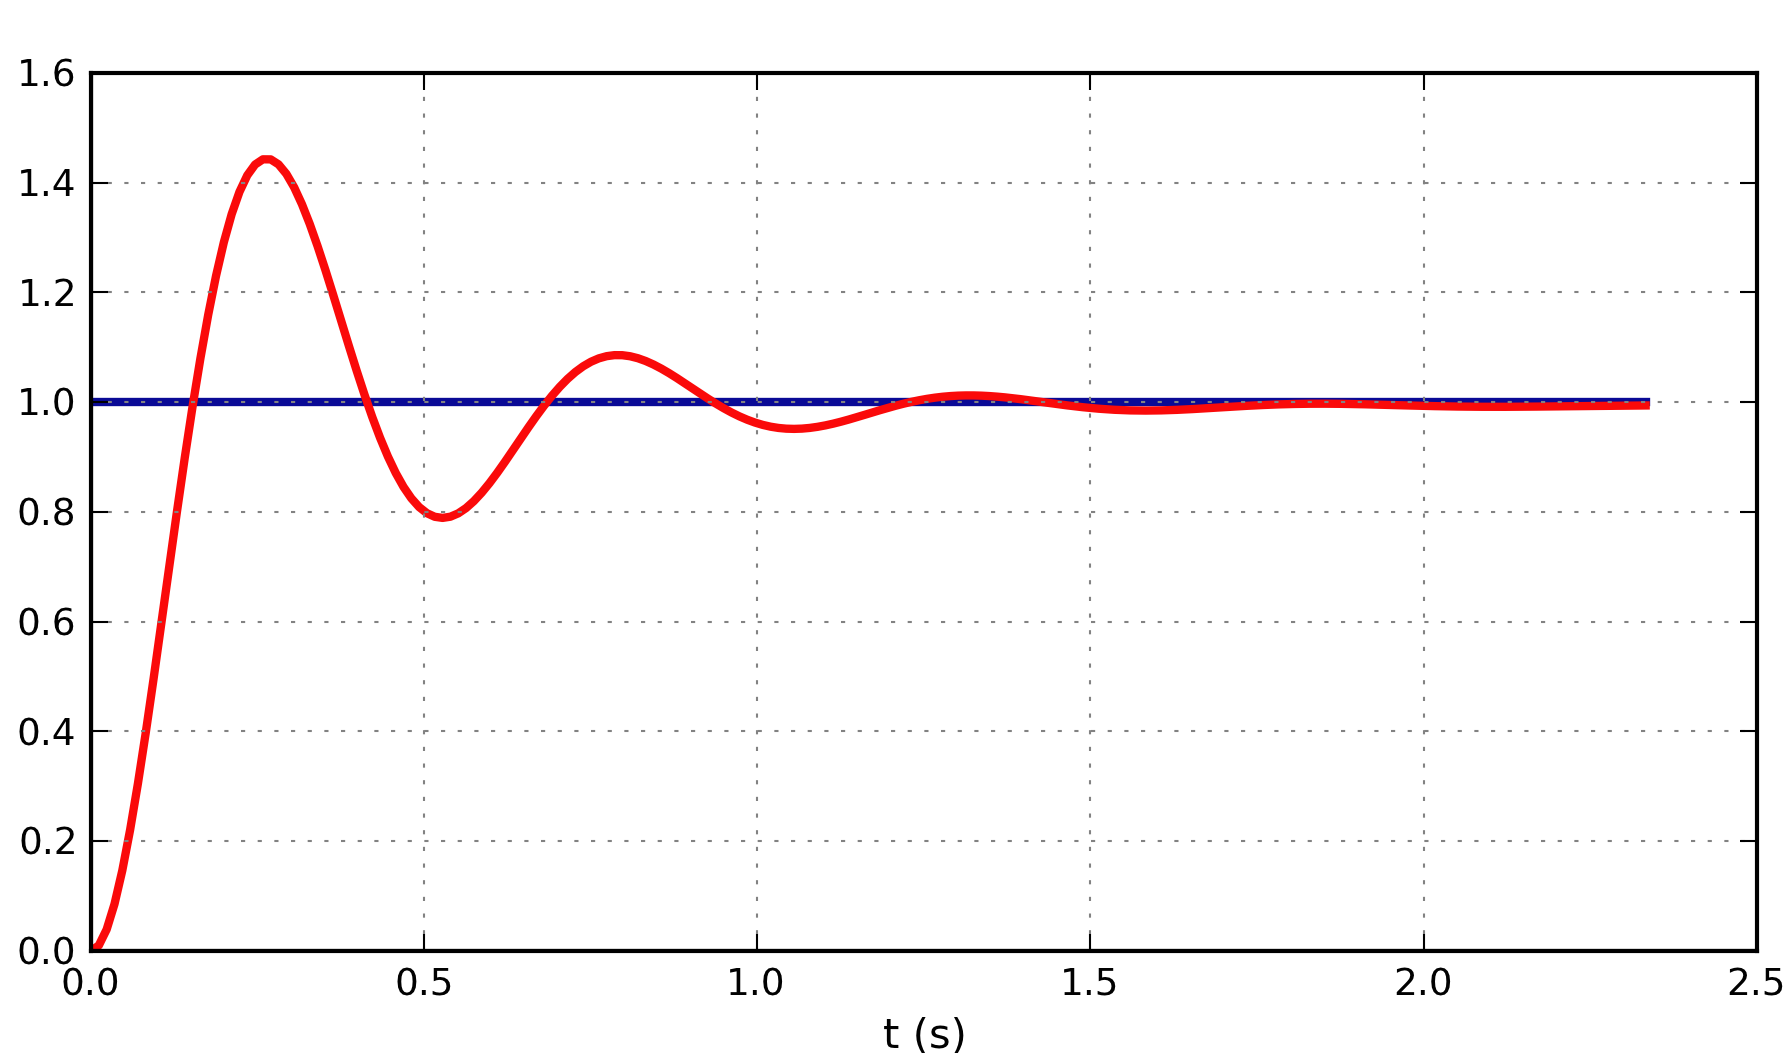
\includegraphics[width=\linewidth]{fig_05a}

$\text{T}_{5\%}$ : \SI{0,88}{s} -- Écart statique : tend $\to$ 0
\end{center}

\end{minipage} \hfill
\begin{minipage}[c]{.46\linewidth}
\begin{center}
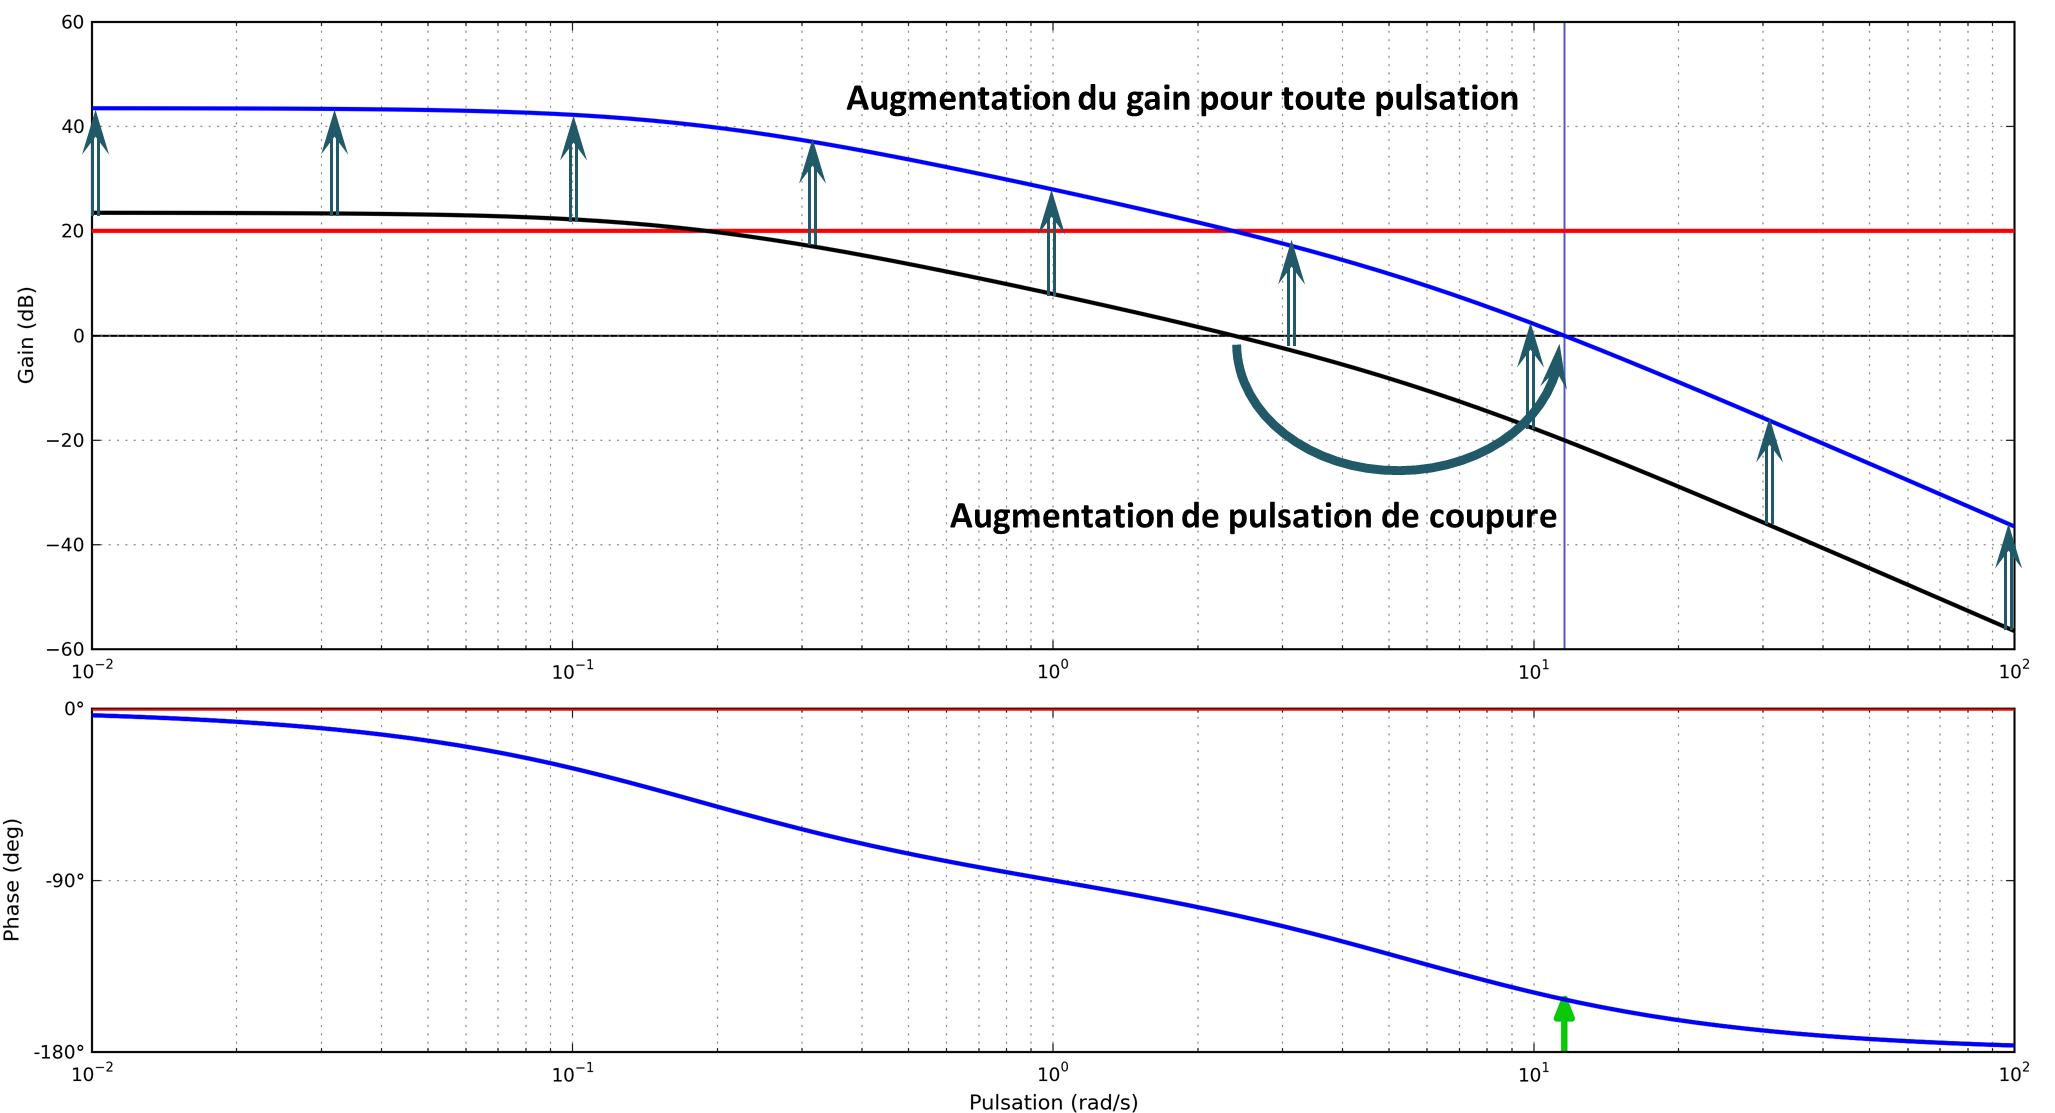
\includegraphics[width=\linewidth]{fig_05b}

Marge de phase 6,43 \degres
\end{center}
\end{minipage} 

\begin{resultat}
~\\
On observe qu'une augmentation du gain proportionnel a pour effet :
\begin{itemize}
\item d'améliorer la précision;
\item d'augmenter la vivacité;
\item d'augmenter le temps de réponse (à partir d'un certain seuil);
\item de diminuer l'amortissement;
\item de diminuer la marge de phase.
\end{itemize}
Pour un système d'ordre supérieur à 2, l'augmentation du gain provoque une marge de phase négative et donc une instabilité du système.
\end{resultat}

\begin{methode} ~\\
\vspace{-1cm}
\begin{multicols}{2}
\textbf{Réglage de la marge de phase :}
\begin{itemize}
\item En utilisant la BO non corrigée, on cherche $\omega_{\SI{0}{dB}}$ tel que $\varphi(\omega_{\SI{0}{dB}})$ respecte la marge de phase souhaitée. 
\item En utilisant BO non corrigée, on calcule $G_{\text{dB}}\left(\omega_{\SI{0}{dB}}\right)$. 
\item On cherche $K_p$ tel que $G_{\text{dB}}\left(\omega_{\SI{0}{dB}}\right)=0$
\end{itemize}
\vspace{.25cm}

\vfill

\textbf{Réglage de la marge de gain :}
\begin{itemize}
\item En utilisant la BO non corrigée, on cherche $\omega_{-180\degres}$ tel que $\varphi(\omega_{-180\degres})=-180\degres$.
\item En utilisant la BO non corrigée, on calcule $G_{\text{dB}}\left(\omega_{-180\degres}\right)$. 
\item On cherche $K_p$ tel qu'on ait la marge de gain souhaitée.
\end{itemize}
\end{multicols}
\end{methode}

\section{Les correcteurs à action intégrale}
\subsection{Le correcteur intégral pur}


\begin{marginfigure}
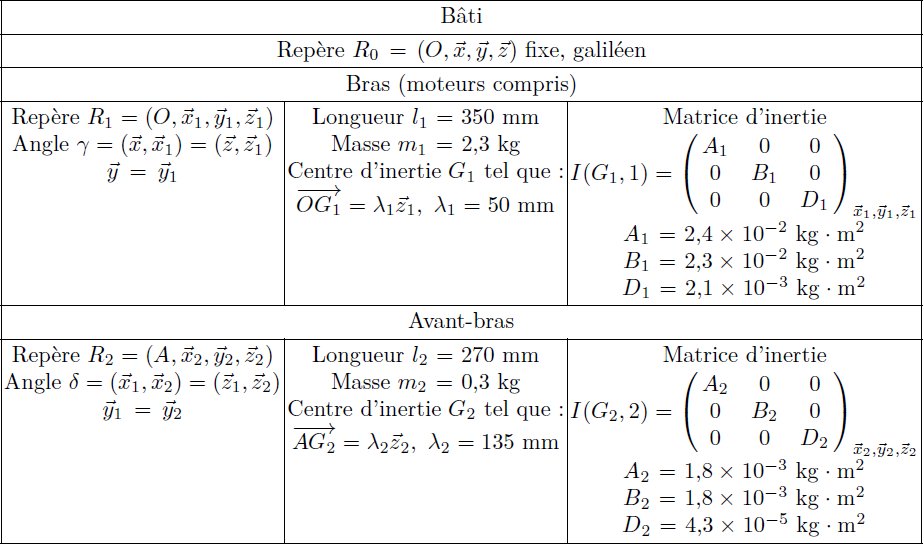
\includegraphics[width=\linewidth]{fig_06}
\end{marginfigure}

\begin{defi}[Correcteur I]
Un correcteur intégral pur a pour fonction de transfert $C(p)=\dfrac{U(p)}{\varepsilon(p)}=\dfrac{1}{T_i p}$.

Dans le domaine temporel on a l'équation de comportement suivante : $u(t)=\dfrac{1}{T_i}\int\limits_0^t \varepsilon (\tau)\text{d}\tau$.
\end{defi}


\begin{resultat} 

\begin{multicols}{2}
\begin{center}
\textbf{Avantages}
\end{center}
Ce correcteur améliore la précision lors de la sollicitation par un échelon car il ajoute une intégration dans la boucle ouverte. 
\begin{center}
\textbf{Inconvénients}
\end{center}
Le déphasage de -90\degres sur tout le spectre de pulsation entraîne une réduction de la marge de phase ce qui peut déstabiliser le système. 
\end{multicols}
\end{resultat}

\subsection{Le correcteur proportionnel intégral}

\begin{marginfigure}
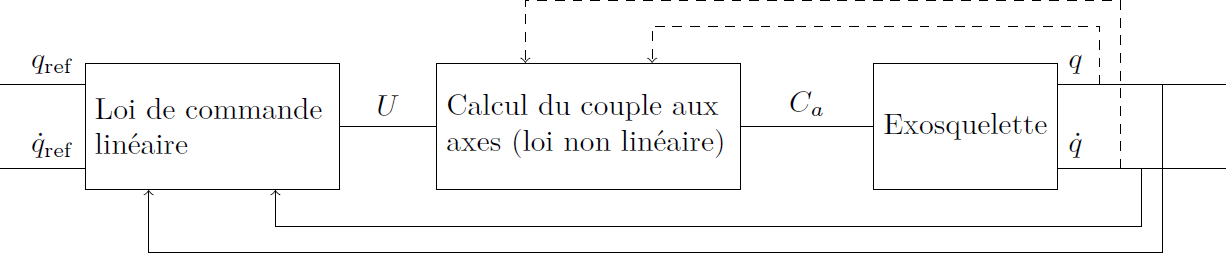
\includegraphics[width=\linewidth]{fig_07}
\end{marginfigure}

\begin{defi}[Correcteur PI]
Un correcteur intégral pur a pour fonction de transfert $C(p)=\dfrac{U(p)}{\varepsilon(p)}=K\left( 1+\dfrac{1}{T_i p}\right)$.
Dans le domaine temporel on a l'équation de comportement suivante : $u(t)=K\left(\varepsilon(t)+\dfrac{1}{T_i}\int\limits_0^t \varepsilon (\tau)\text{d}\tau\right)$.
\end{defi}

En développant on obtient $C(p)=K\dfrac{T_i p+1}{T_i p}$. Ce correcteur augmente donc la classe de la boucle ouverte et donc la précision. Si $K>1$ la pulsation de coupure est augmentée, entraînant ainsi une augmentation de la rapidité du système. Enfin, ce correcteur diminue la phase à basse fréquence. Il faut donc faire en sorte que cette chute de phase n'intervienne pas dans la zone de la pulsation de coupure du système.

\begin{resultat}[Correcteur PI]
\begin{center}
\begin{tabular}{ccccc}
\textbf{augmente l'amortissement,} &&
\textbf{augmente la rapidité,} && 
\textbf{augmente la précision.} \\
\end{tabular}
\end{center}
\end{resultat}



\begin{methode}
\begin{itemize}
\item En utilisant la BO non corrigée, on cherche $\omega_{\SI{0}{dB}}$ tel que $\varphi(\omega_{\SI{0}{dB}})$ respecte la marge de phase souhaitée. 
\item En utilisant la BO non corrigée, on calcule $G_{\text{dB}}\left(\omega_{\SI{0}{dB}}\right)$. 
\item On cherche $K$ tel que $G_{\text{dB}}\left(\omega_{\SI{0}{dB}}\right)=0$
\item La mise en place de l'effet intégral ne doit pas modifier la position de la pulsation de coupure réglée précédemment. Pour cela, il faut donc que $\dfrac{1}{T_i}<< \omega_{\SI{0}{dB}}$. Usuellement on positionne l'action intégrale une décade avant la pulsation réglée. On a donc $T_i=\dfrac{10}{\omega_{\SI{0}{dB}}}$.
\end{itemize}
\end{methode}


\begin{remarque}
Une autre possibilité pour régler $T_i$ est de réaliser \textbf{une compensation de pôle}. Admettons que la FTBO puisse se mettre sous la forme $(1+\tau_1 p)(1+\tau_2 p)$ avec $\tau_1>>\tau_2$. $\tau_1$ ayant pour effet de diminuer la rapidité du système, on pourra prendre $T_i=\tau_1$ afin de supprimer l'effet du pôle associé à $\tau_1$.
\end{remarque}


\section{Le correcteur à avance de phase}

\begin{marginfigure}
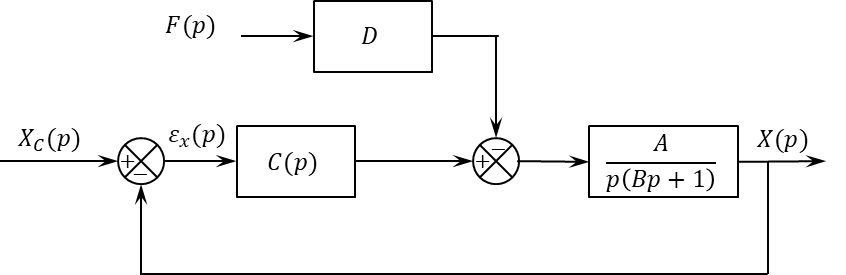
\includegraphics[width=\linewidth]{fig_08}
\end{marginfigure}

\begin{defi}[Correcteur à avance de phase]
Un correcteur à avance de phase a pour fonction de transfert $C(p)=\dfrac{U(p)}{\varepsilon(p)}=K\dfrac{1+a\tau p}{1+\tau p}$ avec $\alpha>1$.
\end{defi}


\begin{resultat}
Ce correcteur permet d'ajouter de la phase pour les pulsations comprises entre $\dfrac{1}{a\tau}$ et $\dfrac{1}{\tau}$. On montre que $\varphi_{\text{max}} = \arcsin \left( \dfrac{a-1}{a+1}\right)$ et ce pour une pulsation $\omega_{\text{max}}=\dfrac{1}{\tau\sqrt{a}}$.
\end{resultat}

\begin{remarque}
On peut prendre $K=\dfrac{1}{\sqrt{a}}$ pour ne pas modifier la valeur du gain à la pulsation où on désire ajouter de la phase. 
\end{remarque}



\subsubsection*{Démonstration}
Pour déterminer $\omega_{\max}$ on pourrait déterminer la pulsation pour laquelle la phase est maximum en résolvant $\dfrac{\text{d}\varphi\left(\omega \right)}{\text{d}\omega}=0$. 
On peut aussi remarquer << graphiquement >> que $\omega_{\text{max}}$ est situé au milieu des deux pulsations de coupures : $\dfrac{1}{2}\left(\log \left(\dfrac{1}{\tau}\right)+\log \left(\dfrac{1}{a\tau}\right)\right)=\log \left(\dfrac{1}{a\tau^2}\right)^{1/2}=\log \left(\dfrac{1}{\tau\sqrt{a}}\right)$ et $\omega_{\text{max}}=\dfrac{1}{\tau\sqrt{a}}$.

D'autre part, il faudrait calculer 
$\varphi\left(\omega_{\text{max}}\right)$...
%
%=\arg(1+aj\tau\omega_{\text{max}})-\arg(1+\tau j\omega_{\text{max}})
%=\arg \left(\dfrac{1+a\tau j\omega_{\text{max}}}{1+\tau j\omega_{\text{max}}} \right)$
%
%$
%=\arg \left(\dfrac{\left(1+a\tau j\omega_{\text{max}}\right)\left(1-\tau j\omega_{\text{max}} \right)}{1-\tau^2 \omega_{\text{max}}^2} \right)$
%
%$
%=\arg \left(1+a\tau j\omega_{\text{max}}-\tau j\omega_{\text{max}} +a\tau^2\omega_{\text{max}}^2 \right)
%$
%
%$
%=\arg \left(\left(1+a\tau^2\omega_{\text{max}}^2\right)+j\left(a\tau \omega_{\text{max}}-\tau \omega_{\text{max}}\right)  \right)$
%
%$
%=\arg \left(2+j\left( \dfrac{a-1}{\sqrt{a}}\right)  \right)$

%\end{demo}


\noindent
\begin{minipage}[c]{.46\linewidth}
Prenons le cas d'un système du second ordre bouclé ($G(p)=\dfrac{100}{\left(p+1\right)^2}$, $a=3,54$, $T=\SI{0,053}{s}$).

\begin{center}
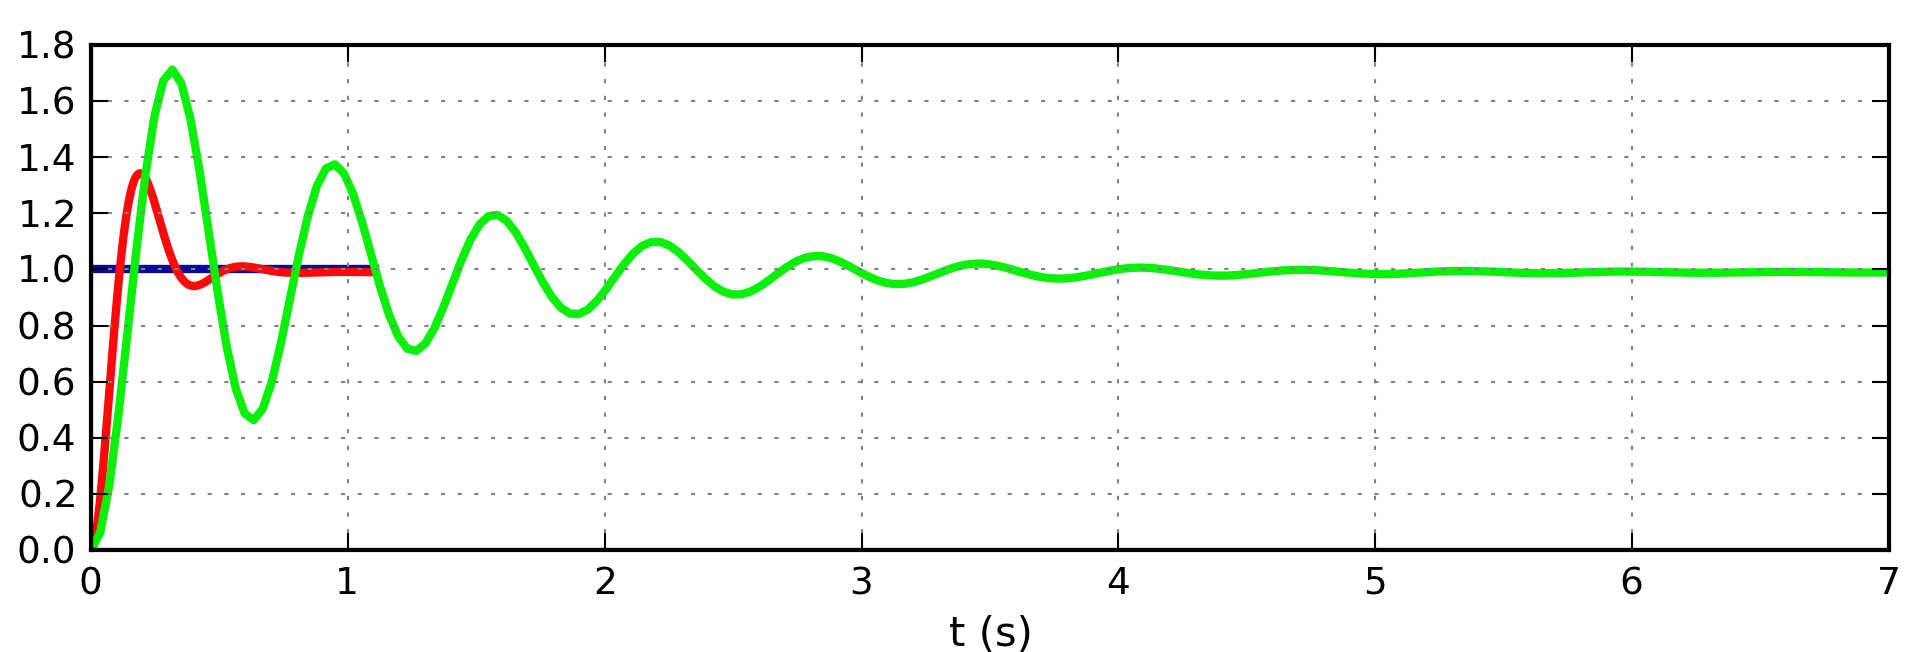
\includegraphics[width=\linewidth]{Avance_BF}

%$\text{T}_{5\%}$ : \SI{0,781}{s} -- Écart statique : 0,07
\end{center}
Ici le correcteur permet une augmentation de la rapidité et un meilleur amortissement.
\end{minipage} \hfill
\begin{minipage}[c]{.46\linewidth}
\begin{center}
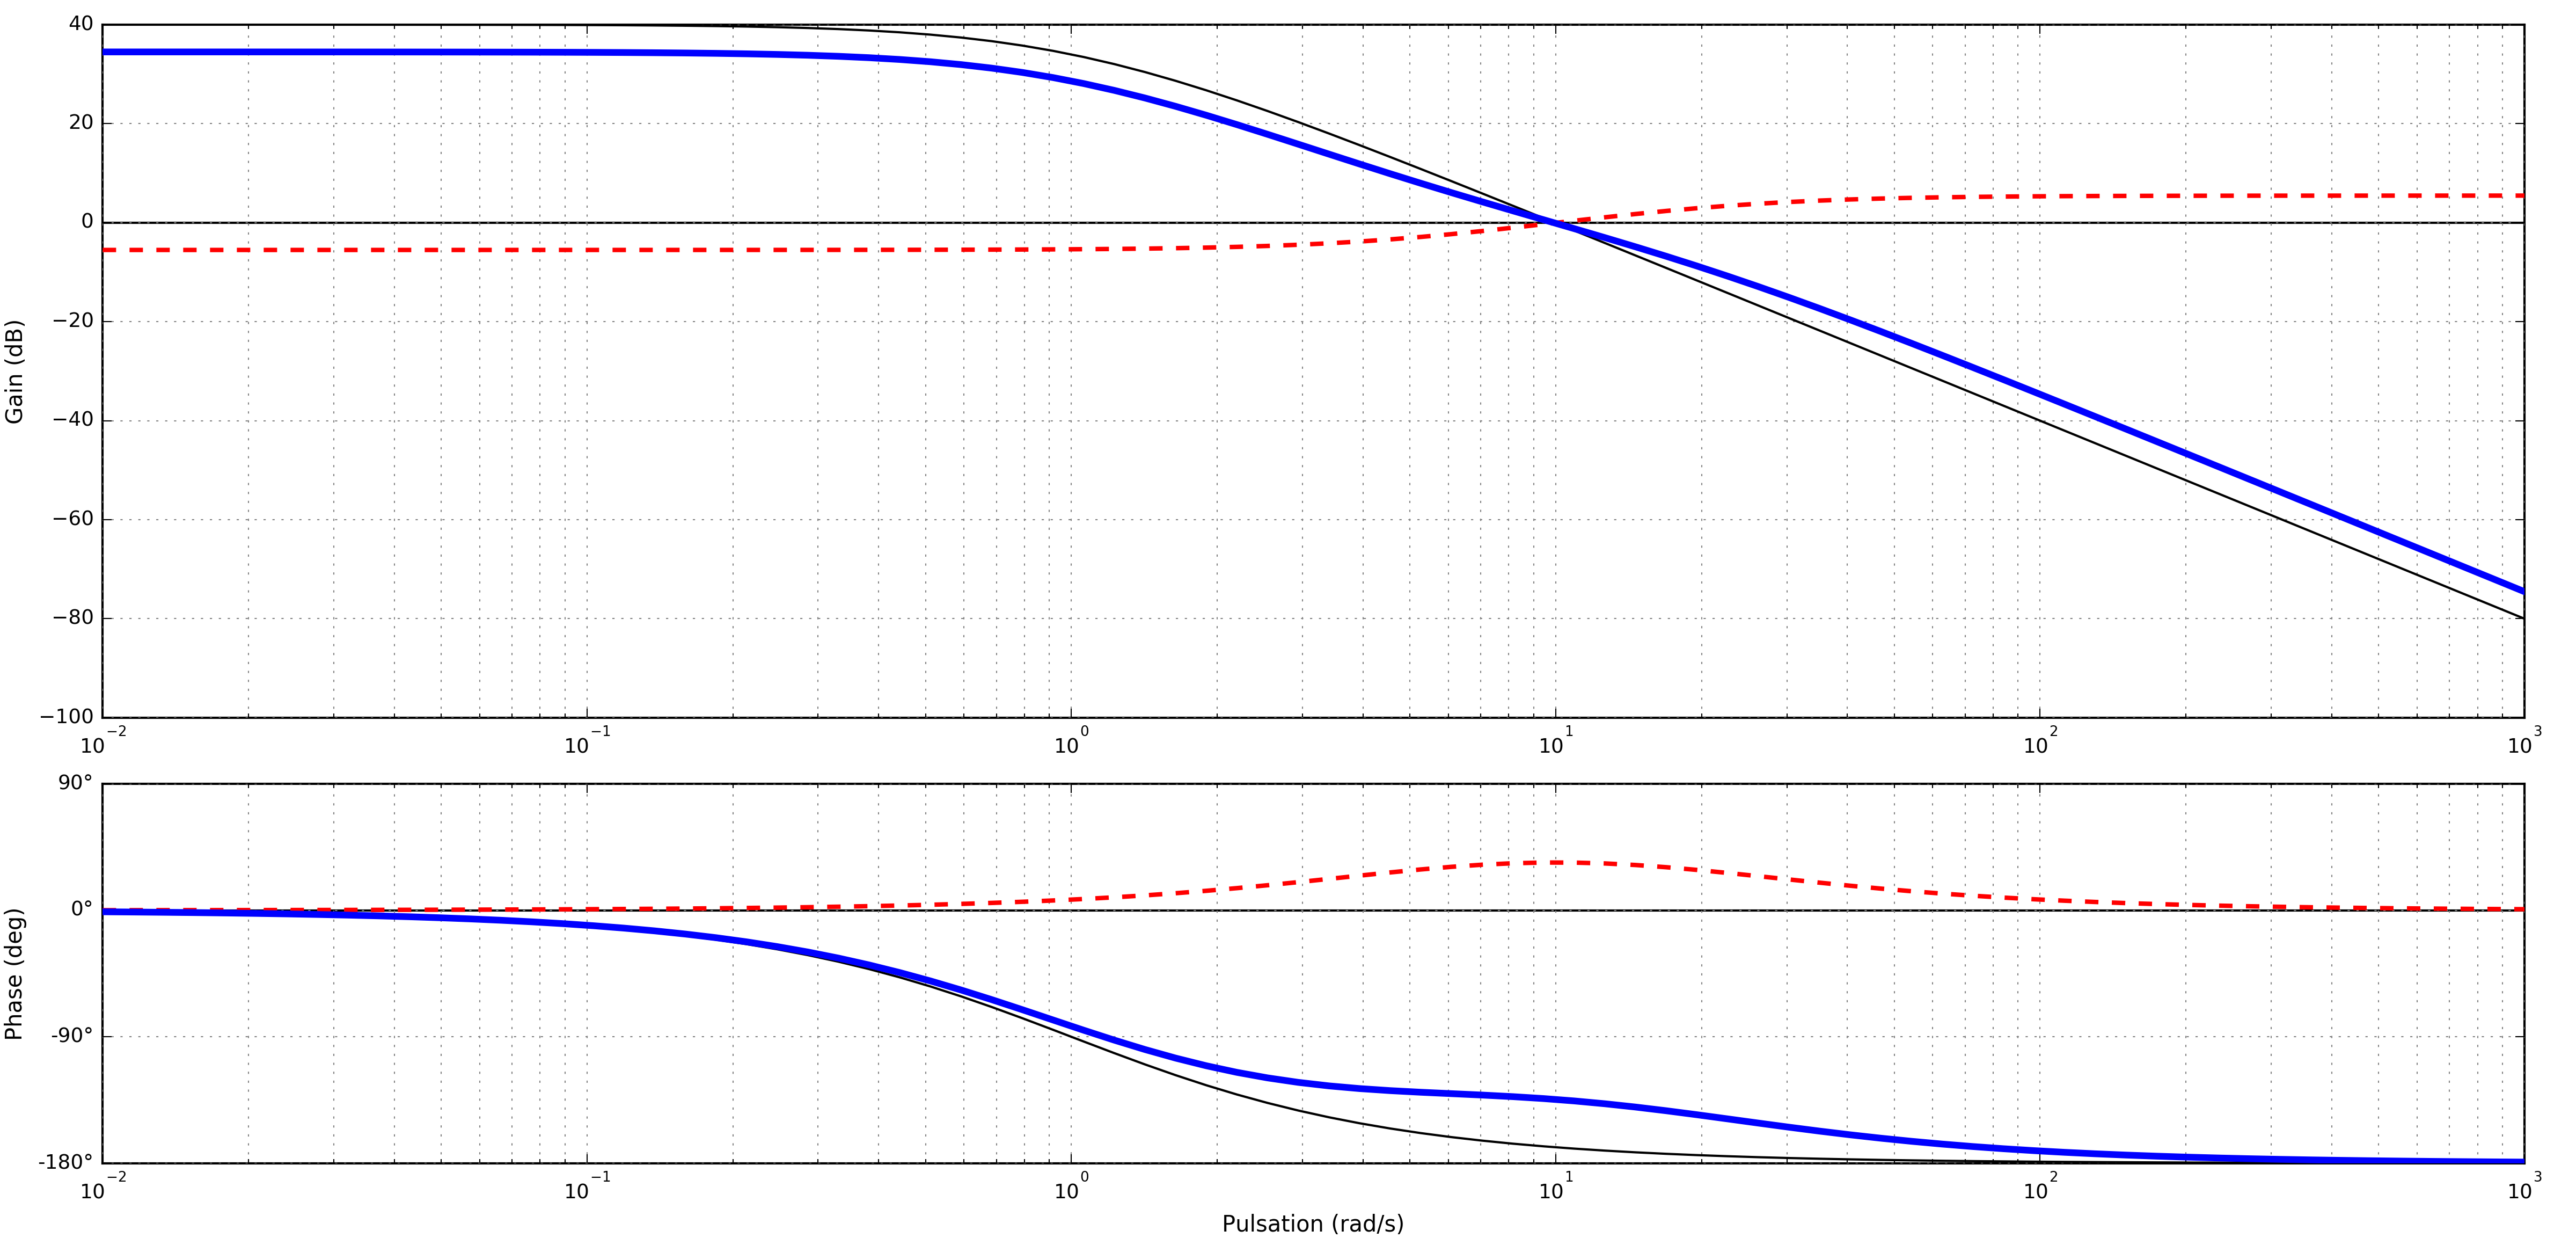
\includegraphics[width=\linewidth]{Avance_Bode_V2}

%Marge de phase 71,94 \degres
\end{center}
\end{minipage} 



\begin{methode}
\begin{itemize}
\item En utilisant la BO non corrigée on cherche $\omega_{\SI{0}{dB}}$ tel que le gain est nul.
\item On calcule $\varphi\left(\omega_{\SI{0}{dB}}\right)$. 
\item On détermine la phase à ajouter. 
\item On calcule $a$. 
\item On calcule $\tau$.
\item On calcule $K$. 
\end{itemize}


\end{methode}


\section{Bilan sur l'influence des correcteurs}
\begin{center}
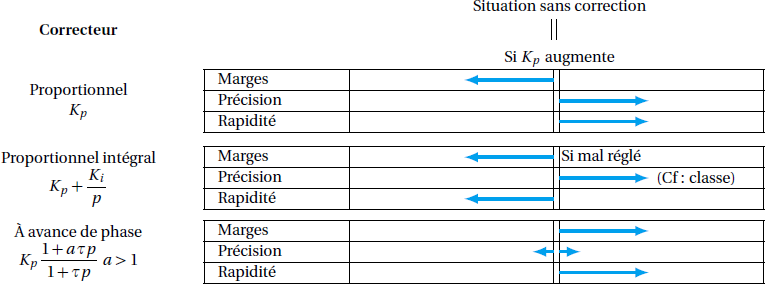
\includegraphics[width=\linewidth]{BilanInfluence}
\end{center}

